%!Mode:: "TeX:UTF-8"
\section{RAID阵列}

独立硬盘冗余阵列(RAID, Redundant Array of Independent Disks),其基本思想就是把多个相对便宜的硬盘组合起来,成为一个硬盘阵列组,使性能达到甚至超过一个价格昂贵、容量巨大的硬盘。根据选择的版本不同,RAID比单颗硬盘有以下一个或多个方面的好处:增强数据集成度,增强容错功能,增加处理量或容量。

\begin{figure}[ht]
	\begin{center}
		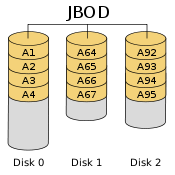
\includegraphics[keepaspectratio,width=0.15\paperwidth]{Pictures/RAID/JBOD.png}
		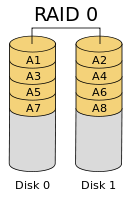
\includegraphics[keepaspectratio,width=0.1\paperwidth]{Pictures/RAID/RAID0.png}
		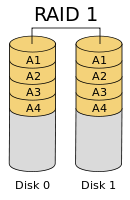
\includegraphics[keepaspectratio,width=0.1\paperwidth]{Pictures/RAID/RAID1.png}
	\end{center}
\end{figure}

\textbf{RAID 0}亦称为带区集。它将两个以上的磁盘串联起来,成为一个大容量的磁盘。在存放数据时,分段后分散存储在这些磁盘中,因为读写时都可以并行处理,所以在所有的级别中,RAID 0的速度是最快的。但是RAID 0既没有冗余功能,也不具备容错能力,如果一个磁盘(物理)损坏,所有数据都会丢失,危险程度与\textbf{JBOD}相当。


\begin{figure}[ht]
	\begin{center}
		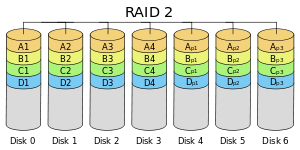
\includegraphics[keepaspectratio,width=0.2\paperwidth]{Pictures/RAID/RAID2.png}
		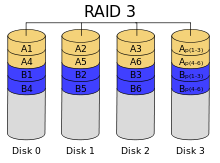
\includegraphics[keepaspectratio,width=0.2\paperwidth]{Pictures/RAID/RAID3.png}
	\end{center}
\end{figure}

两组以上的N个磁盘相互作镜像,在一些多线程操作系统中能有很好的读取速度,理论上读取速度等于硬盘数量的倍数,另外写入速度有微小的降低。只要一个磁盘正常即可维持运作,可靠性最高。\textbf{RAID 1}就是镜像,其原理为在主硬盘上存放数据的同时也在镜像硬盘上写一样的数据。当主硬盘(物理)损坏时,镜像硬盘则代替主硬盘的工作。因为有镜像硬盘做数据备份,所以RAID 1的数据安全性在所有的RAID级别上来说是最好的。但无论用多少磁盘做RAID 1,仅算一个磁盘的容量,是所有RAID中磁盘利用率最低的一个级别。

\begin{figure}[ht]
	\begin{center}
		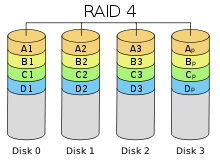
\includegraphics[keepaspectratio,width=0.2\paperwidth]{Pictures/RAID/RAID4.png}
		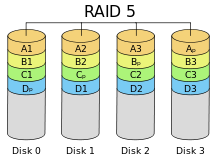
\includegraphics[keepaspectratio,width=0.2\paperwidth]{Pictures/RAID/RAID5.png}
		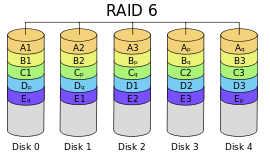
\includegraphics[keepaspectratio,width=0.2\paperwidth]{Pictures/RAID/RAID6.png}
	\end{center}
\end{figure}

\textbf{RAID 2}是RAID 0的改良版,以汉明码的方式将数据进行编码后分区为\textbf{独立的比特},并将数据分别写入硬盘中。因为在数据中加入了错误修正码(ECC,Error Correction Code),所以数据整体的容量会比原始数据大一些,RAID2最少要三台磁盘驱动器方能运作。RAID 2技术实施复杂,在商业环境中很少使用,早已被淘汰。

\begin{figure}[ht]
	\begin{center}
		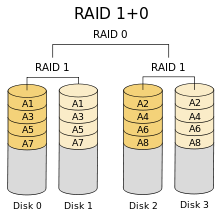
\includegraphics[keepaspectratio,width=0.2\paperwidth]{Pictures/RAID/RAID10.png}
		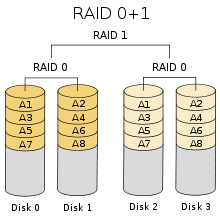
\includegraphics[keepaspectratio,width=0.2\paperwidth]{Pictures/RAID/RAID01.png}
	\end{center}
\end{figure}
\textbf{RAID 3}同RAID 2非常类似,都是将数据条块化分布于不同的硬盘上,区别在于RAID 3使用简单的奇偶校验,并用单块磁盘存放奇偶校验信息。如果一块磁盘失效,奇偶盘及其他数据盘可以重新产生数据;如果奇偶盘失效则不影响数据使用。


\textbf{RAID 4}与RAID 3不同的是它在分区时是以区块为单位分别存在硬盘中(块交织技术,Block interleaving),但每次的数据访问都必须从同比特检查的那个硬盘中取出对应的同比特数据进行核对,由于过于频繁的使用,所以对硬盘的损耗可能会提高。RAID 4使用一块磁盘作为奇偶校验盘,每次写操作都需要访问奇偶盘,这时奇偶校验盘会成为写操作的瓶颈。RAID 4在商业环境中也很少使用,面临淘汰。



\textbf{RAID 5是一种储存性能、数据安全和存储成本兼顾的存储解决方案}。它使用的是Disk Striping(硬盘分区)技术。RAID 5至少需要三颗硬盘,RAID 5不是对存储的数据进行备份,而是把数据和相对应的奇偶校验信息存储到组成RAID5的各个磁盘上,并且奇偶校验信息和相对应的数据分别存储于不同的磁盘上。当RAID5的一个磁盘数据发生损坏后,可以利用剩下的数据和相应的奇偶校验信息去恢复被损坏的数据。RAID 5可以理解为是RAID 0和RAID 1的折衷方案。RAID 5可以为系统提供数据安全保障,但保障程度要比镜像低而磁盘空间利用率要比镜像高。RAID 5具有和RAID 0相近似的数据读取速度,只是因为多了一个奇偶校验信息,写入数据的速度相对单独写入一块硬盘的速度略慢,若使用“回写高速缓存”可以让性能改善不少。同时由于多个数据对应一个奇偶校验信息,RAID 5的磁盘空间利用率要比RAID 1高,存储成本相对较便宜。


与RAID 5相比,RAID 6增加了第二个独立的奇偶校验信息块。两个独立的奇偶系统使用不同的算法,数据的可靠性非常高,即使两块磁盘同时失效也不会影响数据的使用。但RAID 6需要分配给奇偶校验信息更大的磁盘空间,相对于RAID 5有更大的“写损失”,因此“写性能”非常差。较差的性能和复杂的实作方式使得\textbf{RAID 6很少得到实际应用}。同一数组中最多容许两个磁盘损坏。更换新磁盘后,数据将会重新算出并写入新的磁盘中。依照设计理论,RAID 6必须具备四个以上的磁盘才能生效。


RAID 10是先镜射再分区数据,再将所有硬盘分为两组,视为是RAID 0的最低组合,然后将这两组各自视为RAID 1运作。

RAID 01则是跟RAID 10的程序相反,是先分区再将数据镜射到两组硬盘。它将所有的硬盘分为两组,变成RAID 1的最低组合,而将两组硬盘各自视为RAID 0运作。当RAID 10有一个硬盘受损,其余硬盘会继续运作。RAID 01只要有一个硬盘受损,同组RAID 0的所有硬盘都会停止运作,只剩下其他组的硬盘运作,可靠性较低。因此,\textbf{RAID 10远较RAID 01常用}。



\clearpage


